\chapter{Solution definition} \label{chapter:Solution}
%\textbf{roughly 3 pages}

Based on the elicited information from the previous chapter, this chapter examines the specific requirements the artifact must meet. Topics such as the target group, the level of abstraction, the structure of the information presentation, and finally the requirements specification are defined. Following the design science research approach presented in \ref{subsec:GuidelinesDesignScience}, the solution is inferred from the problem statement. Therefore, the artifact must provide a simple explanation which comprehensively explains the blockchain technology and its use cases, thus building an understanding of the technology for a novice audience. 

\section{Target group definition}
As everybody has a different level of knowledge and different information needs, it is crucial to define the audience which the artifact targets. The importance of defining the target group beforehand is made clear both during the expert interviews as well as in section \ref{subsec:BestPracticesDesign}. It also calls for target group definition to design the multimedia instruction in accordance with the user's needs. Therefore, the first question that needs to be answered is how a novice audience is defined. For this purpose, a decision tree of five simple questions is utilized. This decision tree is presented in figure \ref{fig:TargetGroup}. Even though the questions may seem very simple, their straightforward nature (only yes or no questions) helps to quickly identify the target group. This characteristic also makes it easy to use the decision tree during a workshop or a trade fair. While the first and third questions are simple and only show that the person questioned has heard of the terms bitcoin and blockchain, the second and the fourth questions dig deeper into their understanding of these topics. However, replying yes to the fourth question \enquote{Do you know how the blockchain works?} does not prove that the person has in fact fully understood the concepts of the blockchain. Therefore, the fifth question deals with the underlying concepts of cryptoeconomics, which are necessary to fully understand how and why the blockchain technology works.\footcite[Cf.][]{RalphBeckmann_Interview} These five questions allow a simple categorization of the audience. Any person who answers \textit{no} to one of these questions falls into the target group and is therefore considered a novice. It should be noted that the categorization may be faulty if somebody does not know the term cryptoeconomics but still knows the underlying concepts of the three pillars (finance, \ac{IT}, economics/business). For this reason, the fifth question should be asked more elaborately, defining the term cryptoeconomics beforehand.

\begin{figure}
    \centering
    \includesvg[width=\linewidth]{graphics/TargetGroupDefinition.svg}
    \caption{Decision tree for target group definition}
    \label{fig:TargetGroup}
\end{figure}

Once the target audience is defined, the structure of the information presentation needs to be specified. The specification may be divided into two parts: The information flow and the visual presentation of the information, which are described in more detail in the following.

\section{Information presentation} \label{sec:InformationPresentation}
The artifact's purpose is to present an introduction to the blockchain technology and its use cases in a comprehensible way. Therefore, the presentation of the information must be well structured. Taking the suggestion from Beckmann into account (the information should at first be presented and interaction with this information should take place only afterwards),\footcite[Cf.][P115]{RalphBeckmann_Interview} the solution will be divided into two sections: A guided tour, also to be understood as a tutorial, and an overview map which provides access to more detailed explanations of technical concepts. The precise information flow and how the artifact will present and visualize this information is described in the following paragraphs.

\paragraph{Information flow} Since the audience is for the most part unfamiliar with blockchain concepts, the information must be presented in an acceptably abstracted manner. Therefore, most of the technical concepts should be introduced only later, once the general purpose and the underlying concepts of cryptoeconomics have been presented. This means, that the artifact should begin with an explanation of what money is and how it works today, then introduce the mechanics of distributed systems and how they reach a shared state, compare these with and distance them from centralized systems, before proceeding to the third pillar economics/business, where game-theoretic mechanisms such as incentivization are explained. Afterward, the artifact should present some possible use cases with easy-to-grasp examples as this allows the audience to quickly see why blockchain is important and what value it might add to their business. Once these topics have been covered, the characteristic concepts of blockchain should be introduced. These include a more detailed definition of distributed, peer to peer networks, consensus mechanisms (proof of work and proof of stake), cryptographic hash functions, and public and private key cryptography. Overall, it is essential to stay on an abstract level and to present an overview, so that the audience is not overwhelmed by new concepts and that they stay engaged and interested. For a more detailed definition of the information flow, the information flow of existing learning resources is taken as an orientation to include all relevant concepts and terms of the blockchain technology. For this reason, the projects \textit{Blockchaindemo} \& \textit{Coindemo}, \textit{Learn Me A Bitcoin}, and the book \textit{Mastering Bitcoin} are chosen as references, as the visualizations provide a thorough presentation of the relevant topics and because the book is considered one of the most detailed and well-written introductions to blockchain/bitcoin. These projects pursue similar, yet different approaches when introducing the underlying concepts, thus giving insights into how the artifact may be designed. The information flow of these projects is presented in figure \ref{fig:ProcessBC}.\footnote{Due to \textit{Learn Me A Bitcoin}'s unstructured nature, the accompanying guide (instead of the visualization) is taken as the basis for the comparison.} 

\begin{figure}
    \centering
    %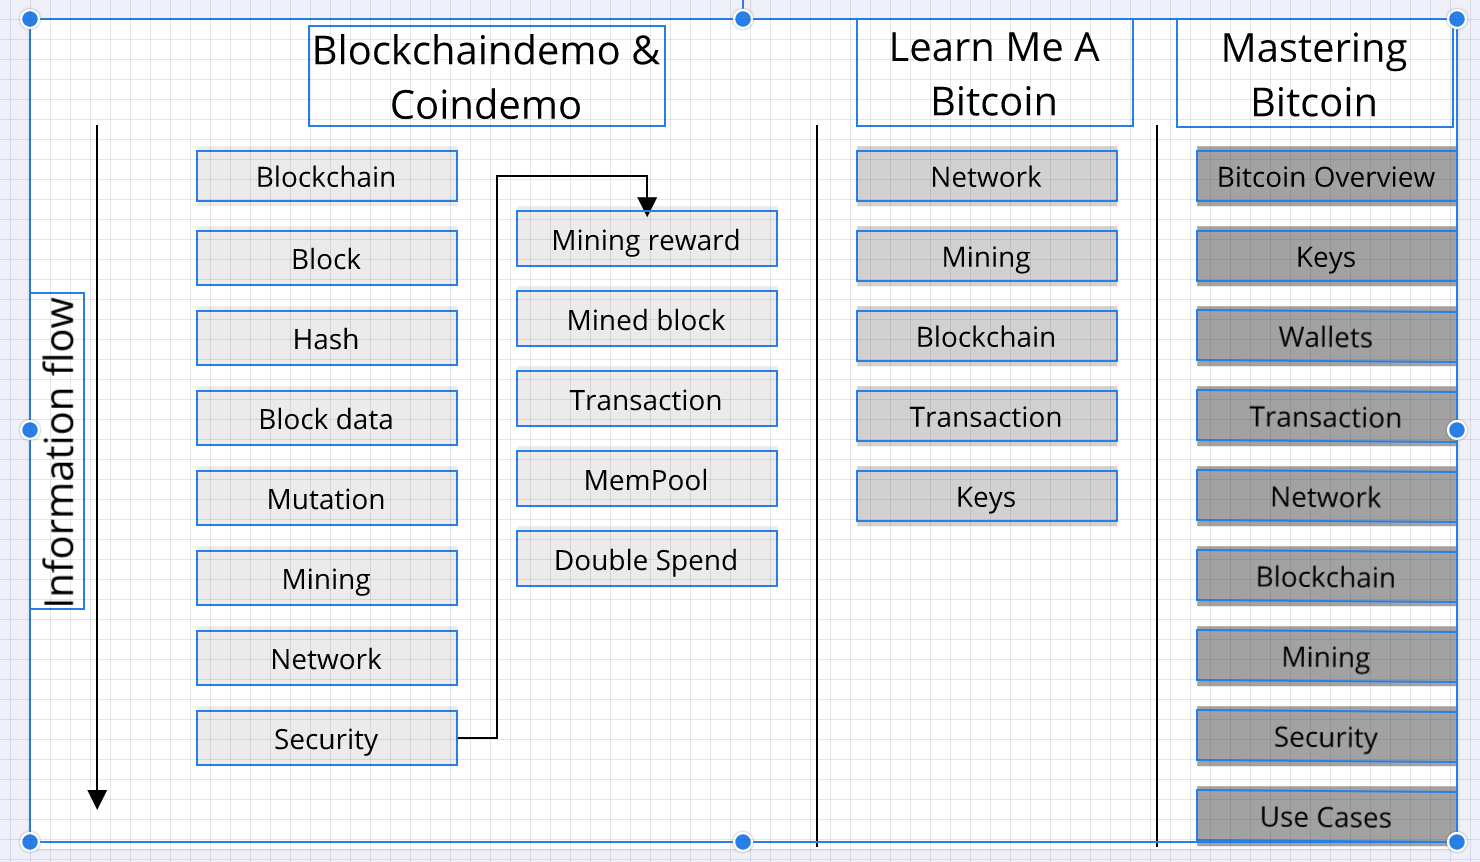
\includegraphics[width=\linewidth]{latex-vorlage_v1.5/graphics/ProcessBC.png}
    \includesvg[width=\textwidth]{graphics/BCExplanation}
    \caption{Comparison of the information flow from \textit{Blockchain}- and \textit{Coindemo}, \textit{Learn Me A Bitcoin} and \textit{Mastering Bitcoin}.}
    \label{fig:ProcessBC}
\end{figure}

The common terms and concepts that all of the presented projects define are: blockchain, mining, transactions, and the peer to peer network. Additionally, two of the three projects describe the role of cryptographic keys and blockchain's security features. However, none present these concepts in the same order as the other, which suggests that the flow of information is less dependent on the technical concepts than on the author's choice and their storytelling style. For this reason, a particular information flow of the more technical concepts cannot be derived from this comparison. However, it has become clear that the concepts and definitions of blockchain, mining, transactions, and peer to peer networking must be included. The artifact will hence discuss these concepts on a relatively high abstraction level during the first section (the guided tour). However, the user is given the possibility to learn about some of the concepts in more detail once the guided tour is finished. They will then be presented with an overview of the major elements of the blockchain technology which, when clicked upon, show additional information. 

\paragraph{Interactivity} As Mayer and other authors have stated, interactivity (if done correctly) provides a way to engage the audience in more meaningful learning.\footcites[Cf.][p.310]{MorenoInteractiveMultimodalLearning2007}[cf.][p.160]{ZhangInteractiveMultimediaBasedELearning2005}[cf.][p.190]{LeeScreenDesignGuidelines1999} The artifact will contain different elements (for navigating, controlling, and manipulating data) which motivate the audience to participate and play with the presented information. One of these elements is the presentation of how a cryptographic hash function works. The user will be able to enter a value and see the corresponding hash value. Similarly, the user will also be able to change the content of a block and see how such a change affects the appended blocks. Such interactions allow the user to explore the technologies actively and thus to learn more deeply. The full list of interactive elements is presented in \ref{sec:ArtifactDesign} as part of the design process. 

%as this interactivity is what is missing in most of the other existing explanations. For this purpose, the artifact will use different interactivity types (presented in \ref{sec:Interactivity}, such as controlling, navigating and manipulating. During the first part, the user interacts with the artifact as they follow the explanation by determining the speed of the presentation. The second part is more open to the user as it allows different concepts to be explored and these concepts will 

\paragraph{Visual information presentation} The findings from \ref{sec:Interactivity}, \ref{sec:GuidelinesMultimediaInstr}, \ref{sec:ExistingSolutions}, as well as from the expert interviews show that information should be presented in an easy-to-understand manner. One possible way to engage the audience in meaningful learning is to use visualizations of the information with which the audience may interact (multimedia principle and interactivity principle).\footcites[Cf.][]{RalphBeckmann_Interview}[cf.][p.1025]{DomagkInteractivitymultimedialearning2010}[cf.][p.311]{MorenoInteractiveMultimodalLearning2007}[cf.][p.290]{Betrancourtanimationinteractivityprinciples2005} For this reason, the artifact will contain different visualizations to support the explanation. One of these visualizations will present a decentralized network as opposed to a centralized network. Another will present how the different blocks are linked with each other. Regarding the style of information presentation, note that the information will be provided in the form of written text. Although the modality principle suggests a different approach (presenting words as speech rather than on-screen text) to distribute the cognitive loads on different sensory channels, this principle is only partially applicable to the situation as the information contains a number of technical terms with which the audience is unfamiliar and which should therefore remain visible.\footcite[Cf.][chapter 6, paragraph 1]{ClarkElearningscienceinstruction2016} Additionally, as this artifact may be used for demonstrations during trade fairs or conferences, a solution with no audio files is preferred for the following reasons: simpler set-up, less equipment necessary, and the possibility to begin a conversation with the partner at any time. To conclude, the visualization's intent is to underline the presented information (in written form) and thus to make the information easier to understand. That is why the graphics used should be simple and pithy. Since graphics and visualizations in addition to text are a tool to foster meaningful learning (multimedia principle), they must be understood as such and hence should be used only in suitable situations. 

\section{Requirements specification} \label{sec:ReqSpec}
While the previous paragraphs have simply described some characteristics the artifact will have, this section formally defines the requirements the artifact must meet. The detailed specification (regarding content, structure, and design) is based on the theoretical principles and insights gained from the literature reviews and expert interviews. It allows for a well-structured and theory-led approach to the design and development phases of the artifact. Where applicable, an arrow ($\rightarrow$) is used to indicate which principles and insights provide the basis for a particular requirement.

\paragraph{Content} The artifact must present the following information: 
\begin{enumerate}[nosep]
\newcounter{foo}
    \item A short overview of cryptoeconomics. This includes the financial aspect (What is money and how does it work?), the \ac{IT} aspect (What are distributed systems? How do they reach a shared state?), and the economics/business aspect (How does game theory apply to this situation and what is incentivization?) $\rightarrow$ \cite{RalphBeckmann_Interview} P86 and P122
    \item A description of a peer to peer network and the nodes within
    \item A blockchain definition 
    \item A differentiation between blockchain, distributed ledger technology and other concepts such as distributed file systems $\rightarrow$ \cite{DanielKaltenbach_Interview} P46 and \cite{RalphBeckmann_Interview} P111
    \item A description of blockchain's use cases $\rightarrow$ \cite{RalphBeckmann_Interview} P113, \cite{DanielKaltenbach_Interview} P14, P57 and \cite{BjoernPaulewicz_Interview} P70, P75
    \item A description of consensus mechanisms and mining methods (proof of work and proof of stake)
    \item A definition of transactions
    \item A definition of smart contracts
    \item A description of cryptographic hash functions
    \item A description of public and private key cryptography
    \item A description of block mutation effects
\setcounter{foo}{\value{enumi}}
\end{enumerate}

\paragraph{Graphical design} The artifact must be designed along the following specifications:
\begin{enumerate}[nosep]
\setcounter{enumi}{\value{foo}}
    \item The text is accompanied by explanatory visualizations $\rightarrow$ multimedia principle and contiguity principle
    \item The graphics are simple symbols and easily identified
    \item Important graphics are visually highlighted $\rightarrow$ cueing
    \item Animations are used to transition between different topics
    \item A uniform gamut of colors is used
    \item Only the relevant information is visible at one time $\rightarrow$ segmenting principle
    \item The overview uses symbols to present every concept
\setcounter{foo}{\value{enumi}}
\end{enumerate}

\paragraph{Structure} The artifact must present the content in the following manner:
\begin{enumerate}[nosep]
\setcounter{enumi}{\value{foo}}
    \item The user may choose to follow a guided tour or to skip it and view an overview of the concepts $\rightarrow$ guided discovery principle and individual differences principle
    \item The guided tour presents small text boxes which contain a description of one specific topic $\rightarrow$ segmenting principle and modality principle
    \item The user follows the tour by clicking through the different text boxes $\rightarrow$ interactivity principle
    \item The user may go back to a previous topic or quit the guided tour by using a site map $\rightarrow$ site map principle
    \item The guided tour serves as an introduction for the second part $\rightarrow$ pretraining principle
    \item The overview provides access to more detailed information on a certain topic $\rightarrow$ segmenting principle
    \item The overall language meets that of a novice audience and uses a friendly, conversational style $\rightarrow$ personalization principle
    \item At the end of the guided tour, the user is directed to the second section: the overview
    \item The user can choose a topic of their interest from the overview for more detailed information $\rightarrow$ segmenting principle
    \item As part of the detailed information, some concepts allow interaction and manipulation of data $\rightarrow$ interactivity principle
    \begin{enumerate}
        \item The user can enter a value into a text field and is presented with the hashed value
        \item The user can create a pair of keys 
        \item The user can mutate a block and see the effects of that change on the blockchain
    \end{enumerate}
\setcounter{foo}{\value{enumi}}
\end{enumerate}

\paragraph{Technology} To ensure its usability and utility, the artifact must fulfill the following technical requirements:
\begin{enumerate}[nosep]
\setcounter{enumi}{\value{foo}}
    \item The solution is location independent, so that it can be presented in various settings
    \item The solution processes user interactions and user input and reacts accordingly
    \item The solution is easily adapted, e.g., to conform to new branding requirements or to include new information
\end{enumerate}


% \subsection{Dashboard content}
% \textit{What exactly should the dashboard visualize?}
% State the requirements that come from the requirements analysis

% \subsection{Technology for dashboard development}
% \begin{itemize}
%     \item What should the technology be able to do? What are the requirements? (Should come from the interviews)
%     \item What possible technologies are there to build a dashboard? 
%     \item Compare these techs with respect to the formulated requirements and choose a solution/combination(?)
% \end{itemize}